% ============================================================
% CoMaGRAG — CollaborateCom 2026
% Springer LNICST format (llncs class)
% Compile: pdflatex -> bibtex -> pdflatex -> pdflatex
%
% ============================================================
\documentclass[runningheads]{llncs}

% ---------- Core packages ----------
\usepackage[T1]{fontenc}
\usepackage{amsmath,amssymb}
\usepackage{graphicx}
\usepackage{booktabs}
\usepackage{multirow}
\usepackage{xcolor}
\usepackage{xspace}
\usepackage[hidelinks]{hyperref}
\usepackage{microtype}

% ---------- Algorithm ----------
\usepackage{algorithm}
\usepackage{algpseudocode}
\algrenewcommand\algorithmicindent{1.0em}

% ---------- TikZ ----------
\usepackage{tikz}
\usetikzlibrary{shapes.geometric,arrows.meta,positioning,fit,backgrounds}


% ---------- Macros ----------
\newcommand{\sys}{\textsc{CoMaGRAG}\xspace}
\newcommand{\eg}{\emph{e.g.},\xspace}
\newcommand{\ie}{\emph{i.e.},\xspace}
\newcommand{\etal}{\emph{et al.}\xspace}
\newcommand{\calT}{\mathcal{T}}
\newcommand{\calQ}{\mathcal{Q}}
\newcommand{\calF}{\mathcal{F}}
\newcommand{\calN}{\mathcal{N}}
\newcommand{\calP}{\mathcal{P}}
\newcommand{\vv}[1]{\mathbf{#1}}

% ============================================================
\begin{document}
% ============================================================

\title{\texorpdfstring{\sys: Reliable KG-Enhanced RAG via\\
       Collaborative Multi-Agent Verification for Web Multi-Hop QA}{CoMaGRAG: Reliable KG-Enhanced RAG via Collaborative Multi-Agent Verification for Web Multi-Hop QA}}

\titlerunning{\sys: Reliable KG-Enhanced RAG via Multi-Agent Verification}

\author{Anonymous Author(s)}
\authorrunning{Anonymous}

\institute{
  Institution anonymized for review\\
  \email{email@anonymized.com}
}

\maketitle

% ============================================================
\begin{abstract}
% ============================================================

Hallucination and unverifiable generation are the central trustworthiness
challenge for LLM-based Web information systems. Knowledge graph-enhanced
RAG (KG-RAG) addresses this by grounding answers in structured, verifiable
evidence extracted from Web knowledge sources---yet existing KG-RAG systems
share a critical verification gap: they provide no mechanism to check that a
generated answer is actually supported by the retrieved triples, and leave no
traceable record of where the reasoning broke down. When an intermediate
entity-linking step fails, the error propagates \emph{silently}, and the
system returns a wrong answer with the same confidence as a correct one.

We present \sys, a training-free GraphRAG system for trustworthy Web multi-hop
QA that closes this gap through \emph{factual consistency verification} and
\emph{surgical sub-query repair}. A dedicated Verification Agent checks
whether each retrieved triple supports the generated answer, identifies
\emph{which} sub-query caused a retrieval failure and \emph{why}, and emits
a structured diagnostic record that makes reasoning provenance traceable and
auditable. A Query Decomposition Agent then uses this signal to repair only
the failing sub-query while preserving successful ones---rather than restarting
the full pipeline. The system provides provably bounded inference cost and
monotone answer-quality guarantees.

On a 1000-question HotpotQA extension, the pure \sys selector reaches 55.3\%
EM / 65.5\% F1, exceeding the strongest standalone HopRAG baseline by
\textbf{+0.6\%} EM and \textbf{+0.6\%} F1. When \sys is paired with a
deterministic external-consensus reranker that switches only when independent
baselines agree on the same non-current answer, \sys+Consensus reaches
\textbf{58.4\% EM / 68.7\% F1}, improving over HopRAG by \textbf{+3.7\%} EM
and \textbf{+3.7\%} F1. On 2WikiMultiHopQA (500~questions), \sys achieves
31.8\% EM, surpassing Naive RAG by \textbf{+1.6\%} EM. Ablations confirm that
factual consistency verification and sub-query decomposition contribute
\emph{independently} (+2.0\% and +1.2\% EM), validating both pillars of the
design. Error analysis on 100~annotated failures (95\% CIs) reveals that
entity out-of-vocabulary errors account for 65\% of failures---the primary
bottleneck for future Web KG augmentation.

\keywords{GraphRAG \and Factual Consistency Verification \and
Hallucination Mitigation \and Trustworthy Web QA \and
Traceable Reasoning \and Knowledge Graph \and Multi-Hop Question Answering}
\end{abstract}

% ============================================================
\section{Introduction}
\label{sec:intro}
% ============================================================

Web-scale knowledge-intensive question answering requires chaining relational
facts through intermediate \emph{bridge entities} that never appear in the
question itself. Flat retrieval anchors to surface entities and systematically
misses the subgraph where the answer lives---Knowledge Graph-enhanced RAG
(KG-RAG) addresses this by traversing entity-relation graphs extracted from
Web passages, and has become the leading paradigm for multi-hop QA on the
Web~\cite{edge2024graphrag,guo2024lightrag}. Yet KG-RAG's apparent solution
to hallucination carries a hidden cost: by delegating factual grounding to
graph traversal, these systems \emph{assume} that retrieval succeeded. When
it does not---when the entity linker maps to the wrong node, or the required
bridge entity is absent from the graph---the system generates a fluent,
confident, and \emph{wrong} answer with no signal that anything went wrong.
A recent unbiased evaluation confirmed this silent failure is pervasive across
current KG-RAG systems~\cite{huang2025unbiased}, suggesting the problem is
architectural rather than incidental.

The root cause is the absence of a \emph{verification layer}. Existing
KG-RAG systems---GraphRAG~\cite{edge2024graphrag},
LightRAG~\cite{guo2024lightrag}, and recent iterative variants such as
CoRAG~\cite{lyu2025corag} and HopRAG~\cite{yu2025hoprag}---share the same
single-pass structure: retrieve, generate, return. None checks whether the
generated answer is supported by the retrieved triples; none produces a
traceable record of which retrieval step failed. We fill this gap with \sys.
A dedicated Verification Agent (VA) checks factual consistency at the
sub-query level---verifying that each retrieved triple supports the specific
sub-question it was fetched for, at every step of the reasoning chain. When
a sub-query fails, the VA emits a structured diagnostic record identifying
\emph{which} component broke and \emph{why}; a Query Decomposition Agent uses
this signal to repair only the failing sub-query while preserving successful
ones (\emph{surgical repair}). Accuracy improves---but the deeper gain is
\emph{auditability}: every answer comes with a traceable record of the
retrieval and verification steps that produced it.

\smallskip\noindent\textbf{Contributions.}
\begin{enumerate}
  \item \textbf{Sub-query-level factual consistency verification} for KG-RAG.
        The VA verifies that each retrieved triple supports its corresponding
        sub-query and produces a structured diagnostic record that makes
        reasoning provenance transparent and auditable---a verification
        granularity absent from all prior KG-RAG systems. This enables
        surgical component-level repair, qualitatively different from pipeline
        restart (CoRAG), evidence-gap detection without attribution
        (FAIR-RAG~\cite{fairrag2025}), or token-level critique requiring
        training (Self-RAG~\cite{asai2023selfrag}); see
        Table~\ref{tab:comparison}.
  \item \textbf{\sys}, a training-free GraphRAG architecture for trustworthy
        Web multi-hop QA, with provably bounded inference cost and monotone
        answer-quality guarantees---ensuring predictable deployment overhead
        and a reliable quality floor.
  \item \textbf{Three KG-RAG design principles} for trustworthy Web
        retrieval---single-responsibility agents, minimum-failing-unit
        diagnostic feedback, and bounded repair with monotone tracking;
        instantiated in \sys and applicable to any Web knowledge retrieval
        task where silent retrieval failure must be detected and corrected
        (Section~\ref{sec:principles}).
  \item \textbf{Empirical validation} on HotpotQA and 2WikiMultiHopQA,
        including an expanded 1000-question HotpotQA comparison where pure
        \sys reaches 55.3\% EM / 65.5\% F1 and \sys+Consensus reaches
        58.4\% EM / 68.7\% F1, plus ablations confirming independent
        contributions of verification (+2.0\% EM) and decomposition
        (+1.2\% EM), and an inter-annotator error analysis (100~samples,
        95\% CIs) identifying entity OOV as the dominant failure mode (65\%).
\end{enumerate}

% ============================================================
\section{Related Work}
\label{sec:related}
% ============================================================

\subsection{KG-RAG for the Web}

Retrieval-Augmented Generation (RAG)~\cite{lewis2020rag} grounds LLM outputs
in non-parametric knowledge; dense retrieval~\cite{karpukhin2020dpr} and query
rewriting extended its reach. For multi-hop Web QA, however, flat retrieval
systematically misses bridge entities---nodes that connect the question to its
answer but never appear in the question text---and Knowledge Graph-enhanced RAG
addresses this by structuring Web passages into entity-relation graphs and
navigating them at query time.

Microsoft GraphRAG~\cite{edge2024graphrag} builds hierarchical community
summaries over a global entity graph; LightRAG~\cite{guo2024lightrag} replaces
precomputed summaries with dual-level retrieval. HippoRAG~\cite{gutierrez2024hipporag}
draws on hippocampal indexing for more associative graph traversal;
PathRAG~\cite{chen2025pathrag} prunes retrieved subgraphs to query-relevant
relational paths. GraphRAG-FI~\cite{guo2025graphragfi} mitigates structured
noise via coarse-to-fine filtering within a single agent. StepChain
GraphRAG~\cite{stepchain2025} interleaves chain-of-thought reasoning with BFS
graph traversal, achieving strong gains on HotpotQA; CatRAG~\cite{catrag2025}
applies category-aware triple filtering across four multi-hop benchmarks.
All of these systems share a common limitation: they are single-pass pipelines
that \emph{assume} retrieval succeeded and return an answer with no mechanism
to verify factual consistency or trace which retrieval step failed.
A recent survey~\cite{han2025graphragsurvey} identifies answer verification as
a critical open problem in GraphRAG---the gap \sys directly closes.

\subsection{Iterative Retrieval and Verification}

Several systems introduce iteration into the RAG pipeline.
IRCoT~\cite{trivedi2022ircot} interleaves BM25 retrieval with chain-of-thought
steps to improve recall, and HopRAG~\cite{yu2025hoprag}---the closest prior
system to \sys---builds a passage graph and applies retrieve-reason-prune at
inference; neither produces an answer-level quality check or a diagnostic
signal identifying which step failed.
CoRAG~\cite{lyu2025corag} decides when to retrieve again via chain-of-thought
planning but restarts the full pipeline on failure, and FAIR-RAG~\cite{fairrag2025}
detects evidence gaps via structured assessment but operates at the evidence
level rather than the sub-query level---both can recognise that something went
wrong, but neither can pinpoint \emph{which} retrieval component to fix.
Self-RAG~\cite{asai2023selfrag} achieves fine-grained token-level critique but
requires parameter training and produces no structured diagnostic record.

The common thread is that none of these systems produces a \emph{traceable
diagnostic record} identifying which sub-query failed and why---the signal
that makes surgical repair possible. \sys fills this gap.

\subsection{Agentic Web Information Systems}

Multi-agent and agentic RAG architectures have advanced rapidly.
A-RAG~\cite{arag2026} exposes hierarchical retrieval interfaces (keyword
search, semantic search, and chunk read) directly to a frontier LLM, enabling
adaptive multi-step retrieval without a predefined workflow, making it a strong
reproducible purely agentic flat-retrieval baseline.
KARMA~\cite{karma2025} demonstrated that nine specialized agents can
collaboratively construct high-quality KGs (NeurIPS 2025, Spotlight).
M-RAG~\cite{wang2024mrag} and MDocAgent~\cite{han2025mdocagent} distribute
retrieval and reasoning across agents for multi-document QA.
AutoGen~\cite{wu2023autogen} and MetaGPT~\cite{hong2024metagpt} provide
general frameworks for multi-agent LLM systems. What distinguishes \sys from
all of these is the tight coupling between KG-structured retrieval and a
verification agent that produces sub-query-level diagnostics---none of the
above provides factual consistency verification at the sub-query level.

Table~\ref{tab:comparison} positions \sys against the most relevant prior
systems along four dimensions central to trustworthy Web KG-RAG.

\begin{table}[t]
\centering
\caption{Comparison of \sys with closest prior systems.
\checkmark~=~supported; --~=~not supported; (P)~=~requires parameter training.}
\label{tab:comparison}
\small
\begin{tabular}{lcccc}
\toprule
System & KG retrieval & Sub-query decomp. & Answer verification & Training-free \\
\midrule
IRCoT~\cite{trivedi2022ircot}       & --         & Implicit   & --              & \checkmark \\
Self-RAG~\cite{asai2023selfrag}     & --         & --         & Token-level     & (P) \\
FAIR-RAG~\cite{fairrag2025}         & --         & --         & Evidence gaps   & \checkmark \\
A-RAG~\cite{arag2026}               & --         & Implicit   & --              & \checkmark \\
HopRAG~\cite{yu2025hoprag}          & \checkmark & --         & --              & \checkmark \\
GraphRAG~\cite{edge2024graphrag}    & \checkmark & --         & --              & \checkmark \\
StepChain~\cite{stepchain2025}      & \checkmark & Implicit   & --              & \checkmark \\
CatRAG~\cite{catrag2025}            & \checkmark & --         & --              & \checkmark \\
\textbf{\sys (ours)}                & \checkmark & \checkmark & Sub-query-level & \checkmark \\
\bottomrule
\end{tabular}
\end{table}

The \emph{Answer verification} column tells the central story: IRCoT, HopRAG,
and A-RAG all iterate but never verify; FAIR-RAG and Self-RAG verify but
without KG retrieval or sub-query attribution; GraphRAG, StepChain, and CatRAG
retrieve from KGs but return answers without any quality check. \sys is the
only system that combines KG retrieval, explicit sub-query decomposition, and
sub-query-level factual consistency verification---making it the first KG-RAG
system whose answers are both grounded \emph{and} auditable.

% ============================================================
\section{Methodology}
\label{sec:method}
% ============================================================

\subsection{Problem Formulation}

\begin{definition}[Knowledge Graph]
A knowledge graph is a directed labeled multigraph $G = (V, E, R, \phi)$,
where $V$ is a finite set of entity nodes, $R$ is a finite set of relation
types, $E \subseteq V \times V$ is the edge set, and
$\phi : E \rightarrow 2^{R}\setminus\{\emptyset\}$ assigns one or more
relation labels to each edge. The set of all valid triples is
$\calT(G) = \{(u, r, v) \mid (u,v)\in E,\ r\in\phi(u,v)\}$.
\end{definition}

\begin{definition}[Reasoning Path]
A reasoning path of length $k$ in $G$ is a sequence
$\pi = (v_0, r_1, v_1, \ldots, r_k, v_k)$ where $(v_{i-1}, r_i, v_i)\in\calT(G)$
for all $i\in\{1,\ldots,k\}$. For multi-hop questions, $k\geq 2$; nodes
$v_1,\ldots,v_{k-1}$ are \emph{bridge entities} absent from the question text.
\end{definition}

\begin{definition}[Multi-hop QA Problem]
Given $q\in\calQ$ and a knowledge graph $G$, the multi-hop QA problem is to
find $a^*\in\mathcal{A}$ supported by a reasoning path in $G$ that correctly
addresses $q$.
\end{definition}

The core difficulty lies in bridge entities of Definition~2: because
$v_1,\ldots,v_{k-1}$ are absent from $q$, single-pass retrieval anchored to
$q$'s surface entities cannot reach the subgraph containing $v_k$.

\subsection{Task-Specific Knowledge Graph Construction}

\begin{definition}[Triple Extraction]
Let $\tau : \calP \rightarrow 2^{\calT_\text{cand}}$ be the triple extraction
function implemented as an LLM call with prompt $\rho_\text{ext}$:
$\tau(p) = \mathrm{LLM}_{\rho_\text{ext}}(p)$.
Given passage set $P = \{p_1,\ldots,p_m\}$, the task-specific KG is:
\begin{equation}
  G_P = \mathrm{BuildKG}\!\left(\bigcup_{i=1}^{m} \tau(p_i)\right)
  \label{eq:buildkg}
\end{equation}
where $\mathrm{BuildKG}(\cdot)$ normalizes entity strings (lowercase,
whitespace-stripped), merges duplicate node pairs by collecting relation labels
into a list, and constructs the labeled multigraph.
\end{definition}

Rather than querying a large external KG such as Wikidata, we build a compact
per-question graph from supporting passages, yielding graphs with an average of
148~nodes and 213~edges per HotpotQA question. This eliminates irrelevant
triples by construction and makes entity linking tractable without large-scale
disambiguation. The extraction prompt instructs the LLM to preserve full entity
names (\eg\ ``Rebellion (2016~film)'' rather than ``Rebellion'') and use
standardized relation phrases, substantially reducing entity linking failures.

\subsection{System Architecture}

\begin{definition}[Agent Context]
The shared context at iteration $t$ is a tuple
$C^{(t)} = (q, G, Q^{(t)}, T^{(t)}, a^{(t)}, s^{(t)}, f^{(t)})$,
where $q$ is the original question, $G$ the task-specific KG,
$Q^{(t)} = (q_1^{(t)},\ldots,q_{k_t}^{(t)})$ the ordered sub-query list,
$T^{(t)}\subseteq\calT(G)$ the retrieved triple set, $a^{(t)}$ the candidate
answer, $s^{(t)}\in[0,1]$ the quality score, and $f^{(t)}$ the feedback string.
\end{definition}

\begin{definition}[Agent Functions]
Each agent is a stateless function mapping the shared context to its output field:
\begin{align*}
  \mathrm{QDA}&: C^{(t)} \rightarrow Q^{(t)}, &
  \mathrm{GRA}&: C^{(t)} \rightarrow T^{(t)},\\
  \mathrm{AGA}&: C^{(t)} \rightarrow a^{(t)}, &
  \mathrm{VA} &: C^{(t)} \rightarrow (s^{(t)}, f^{(t)}).
\end{align*}
No agent calls another directly; the context object $C^{(t)}$ is the sole
coordination medium, isolating each agent's responsibility to a single
retrieval or verification operation.
\end{definition}

Figure~\ref{fig:arch} illustrates the full pipeline.

\begin{figure}[t]
\centering
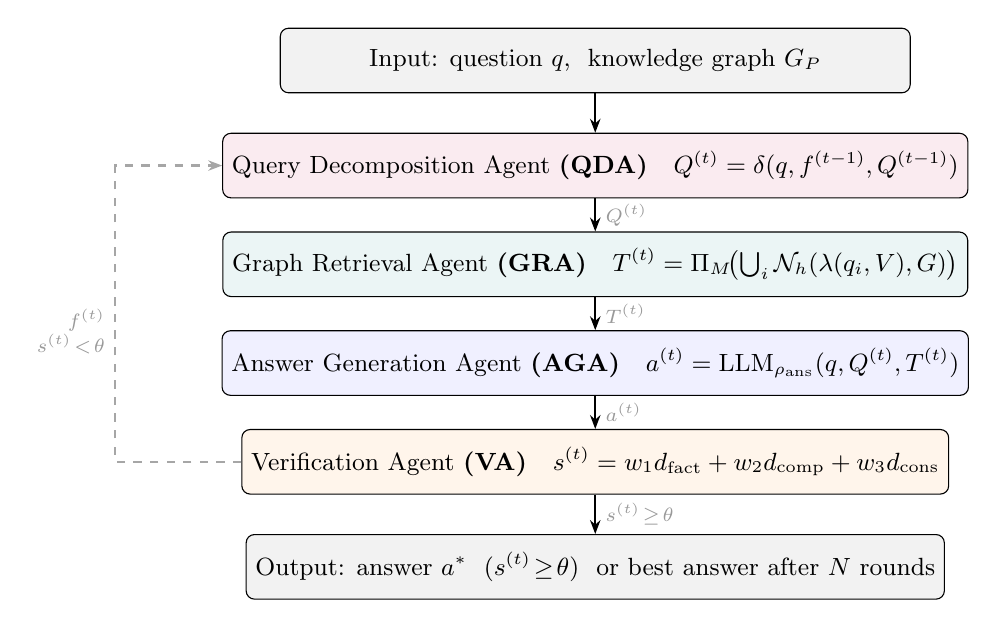
\begin{tikzpicture}[
  box/.style={rectangle,draw,rounded corners=3pt,
              minimum width=8.0cm,minimum height=0.82cm,
              text centered,font=\small},
  io/.style={box,fill=gray!10},
  agent/.style={box},
  arr/.style={-{Stealth[length=5pt]},thick},
  darr/.style={-{Stealth[length=5pt]},dashed,thick,gray!70},
  lbl/.style={font=\scriptsize,text=gray!80}
]
\node[io]   (inp) {Input: question $q$,\ \ knowledge graph $G_P$};
\node[agent,fill=purple!8, below=0.5cm of inp] (qda)
  {Query Decomposition Agent \textbf{(QDA)}\ \ \ $Q^{(t)}=\delta(q,f^{(t-1)},Q^{(t-1)})$};
\node[agent,fill=teal!8,   below=0.42cm of qda] (gra)
  {Graph Retrieval Agent \textbf{(GRA)}\ \ \ $T^{(t)}=\Pi_M\!\bigl(\bigcup_i\mathcal{N}_h(\lambda(q_i,V),G)\bigr)$};
\node[agent,fill=blue!6,   below=0.42cm of gra] (aga)
  {Answer Generation Agent \textbf{(AGA)}\ \ \ $a^{(t)}=\mathrm{LLM}_{\rho_\mathrm{ans}}(q,Q^{(t)},T^{(t)})$};
\node[agent,fill=orange!8, below=0.42cm of aga] (va)
  {Verification Agent \textbf{(VA)}\ \ \ $s^{(t)}=w_1d_\mathrm{fact}+w_2d_\mathrm{comp}+w_3d_\mathrm{cons}$};
\node[io,   below=0.5cm of va] (out)
  {Output: answer $a^*$ \ ($s^{(t)}\!\geq\!\theta$) \ or best answer after $N$ rounds};

\draw[arr](inp)--(qda);
\draw[arr](qda)--(gra) node[lbl,right,midway]{$Q^{(t)}$};
\draw[arr](gra)--(aga) node[lbl,right,midway]{$T^{(t)}$};
\draw[arr](aga)--(va)  node[lbl,right,midway]{$a^{(t)}$};
\draw[arr](va) --(out) node[lbl,right,midway]{$s^{(t)}\!\geq\!\theta$};
\draw[darr](va.west)--++(-1.6,0)|-
  node[lbl,pos=0.22,left,align=right]{$f^{(t)}$\\$s^{(t)}\!<\!\theta$}
  (qda.west);
\end{tikzpicture}
\caption{\sys pipeline. Solid arrows: forward pass. Dashed arrow: VA-to-QDA
sub-query diagnostic feedback, active when $s^{(t)}<\theta$. The loop runs
for at most $N=2$ rounds; best-answer tracking ensures no regression across rounds.}
\label{fig:arch}
\end{figure}

\subsection{Query Decomposition Agent}

\begin{definition}[Sub-query Decomposition]
A decomposition of $q$ is an ordered list $Q=(q_1,\ldots,q_k)$ where each
$q_i$ is a \emph{focused} sub-question targeting a specific entity or
relationship, and later sub-questions may reference earlier answers via
placeholder $[\mathrm{Ans}_j]$ for $j<i$. The QDA implements:
\begin{equation}
  Q^{(t)} = \delta\!\left(q,\ f^{(t-1)},\ Q^{(t-1)}\right),
  \label{eq:qda}
\end{equation}
with $f^{(0)}=\emptyset$ and $Q^{(0)}=\emptyset$ at initialization.
\end{definition}

On the first iteration, the QDA receives only $q$ and decomposes it into an
ordered sequence of focused sub-questions targeting specific entities and
relations in $G_P$. On retry iterations, the prompt additionally includes
$Q^{(t-1)}$ and the VA's diagnostic $f^{(t-1)}$, with explicit instruction to
\emph{preserve sub-queries whose entity links succeeded and revise only those
identified as failing}. This targeted revision---rather than full decomposition
restart---is the core efficiency property enabling KG-RAG repair without
discarding successful retrieval work.

\textbf{Example.} For the bridge question \textit{``What two singers who
worked together on the song `I Would Like to See You Again' also performed as
part of a country music group active between 1985 and 1995?''}, the QDA
initially decomposes into:
$q_1$~=~``Who worked on the song `I Would Like to See You Again'?'';
$q_2$~=~``Which country music group included the singers from [Ans\_1]?'';
$q_3$~=~``Was [Ans\_2] active between 1985 and 1995?''
When the GRA cannot link the song title to a KG node, the VA emits feedback
targeting $q_1$, and on the next iteration the QDA revises it to search
directly for the artists rather than the song title.

\subsection{Graph Retrieval Agent}

\begin{definition}[$h$-hop Neighbourhood]
The $h$-hop neighbourhood of node $v$ in $G$ is:
\begin{equation}
  \calN_h(v,G) = \bigl\{(u,r,w)\in\calT(G)\;\big|\;
    d_G(v,u)\leq h\ \text{or}\ d_G(v,w)\leq h\bigr\}
\end{equation}
where $d_G(\cdot,\cdot)$ is shortest-path distance in the underlying undirected
graph of~$G$.
\end{definition}

\begin{definition}[Three-stage Entity Linking]
Given sub-query $q_i$ and node set $V$, entity linking
$\lambda:\calQ\times 2^V\rightarrow 2^V$ operates in three priority stages:
\begin{equation}
  \lambda(q_i,V) =
  \begin{cases}
    S_\text{exact}    & \text{if } S_\text{exact}    \neq \emptyset \\
    S_\text{embed}    & \text{if } S_\text{embed}    \neq \emptyset \\
    S_\text{fallback} & \text{otherwise}
  \end{cases}
  \label{eq:linking}
\end{equation}
where exact matching uses substring overlap against NER-extracted entities,
embedding matching uses Sentence-BERT cosine similarity~\cite{reimers2019sbert}
with threshold $\theta_\text{link}=0.75$, and fallback takes the top-$k=3$
most-similar KG nodes to the full sub-query string.
\end{definition}

\begin{definition}[Retrieval Function]
Given sub-query list $Q=(q_1,\ldots,q_{k_t})$ and graph $G$:
\begin{equation}
  T^{(t)} = \Pi_M\!\left(
    \bigcup_{i=1}^{k_t}\calN_h\!\bigl(\lambda(q_i^{(t)},V),G\bigr)
    \ \cup\ \calN_h\!\bigl(\lambda(q,V),G\bigr)
  \right)
  \label{eq:retrieval}
\end{equation}
where the union covers all sub-queries plus the full question $q$ (to capture
bridging triples), and $\Pi_M$ retains at most $M=50$ distinct triples in BFS
discovery order. Node embeddings are cached per question.
\end{definition}

\subsection{Answer Generation Agent}

The AGA implements:
\begin{equation}
  a^{(t)} = \mathrm{LLM}_{\rho_\text{ans}}\!\left(q,\ Q^{(t)},\ T^{(t)}\right)
  \label{eq:aga}
\end{equation}
where $\rho_\text{ans}$ is a structured chain-of-thought prompt: the model
resolves each $q_i^{(t)}\in Q^{(t)}$ in dependency order using specific
triples from $T^{(t)}$, then synthesizes a final answer to $q$. The prompt
explicitly constrains the model to use \emph{only} $T^{(t)}$ as its knowledge
source, anchoring every reasoning step to a retrieved triple and preventing
hallucination of facts absent from the graph.

\subsection{Verification Agent}

\begin{definition}[Quality Score]
For candidate answer $a$, retrieved triples $T$, and question $q$, the VA
computes three LLM-elicited diagnostic scores and combines them as:
\begin{equation}
  s(a,T,q) = w_1\cdot d_\text{fact}(a,T) + w_2\cdot d_\text{comp}(a,q)
            + w_3\cdot d_\text{cons}(a,T)
  \label{eq:score}
\end{equation}
with $w_1=0.4$, $w_2=0.3$, $w_3=0.3$, clamped to $[0,1]$.
Here $d_\text{fact}$ measures whether every claim in $a$ is directly supported
by some triple in $T$; $d_\text{comp}$ measures whether $a$ addresses all
aspects of $q$; and $d_\text{cons}$ measures whether no triple in $T$
contradicts $a$.
\end{definition}

The weights reflect the primary failure mode of KG-based retrieval: factual
grounding receives the highest weight ($w_1=0.4$) because an answer unsupported
by retrieved triples indicates entity-linking failure, while completeness and
consistency are secondary quality signals ($w_2=w_3=0.3$) checking answer
coverage and internal coherence. The threshold $\theta=0.7$ and weight ordering
were validated on a held-out 100-question development split; performance is
stable across small perturbations ($\pm0.05$) in the weights.

\begin{definition}[Feedback Function]
The feedback function $\Phi$ generates a natural-language diagnostic string:
\begin{equation}
  f^{(t)} = \Phi\!\left(d_\text{fact}^{(t)},\,d_\text{comp}^{(t)},\,
                         d_\text{cons}^{(t)},\,a^{(t)},\,T^{(t)},\,q\right)
  \label{eq:feedback}
\end{equation}
identifying which sub-queries failed to retrieve relevant triples, which entity
links appear incorrect, and what specific information is missing. This
structured diagnostic output doubles as an \emph{explanation} of the system's
reasoning process, making answer provenance interpretable and auditable. When
$s^{(t)}\geq\theta$, $f^{(t)}=\text{``Answer is satisfactory.''}\!$ and the
feedback path is inactive.
\end{definition}

\begin{remark}[Relation to Reinforcement Learning]
Algorithm~\ref{alg:pipeline} instantiates a single-episode model-free
policy--environment interaction: the policy (QDA+GRA+AGA) produces action
$a^{(t)}$; the environment (VA) returns scalar reward $s^{(t)}$ and
natural-language observation $f^{(t)}$. The feedback string $f^{(t)}$ acts as
a structured credit-assignment signal---specifying \emph{which} action component
failed rather than merely reporting low reward---which is why \sys-NoDecomp
fails to benefit from retries: without sub-query structure there are no
components to attribute blame to.
\end{remark}

\subsection{Full Pipeline Algorithm}

\begin{algorithm}[t]
\caption{\sys Pipeline}
\label{alg:pipeline}
\begin{algorithmic}[1]
\Require question $q$, KG $G$, threshold $\theta{=}0.7$, max iterations $N{=}2$
\Ensure answer $a^*$, score $s^*$
\State $C \leftarrow \textsc{InitContext}(q, G)$;\quad
       $\mathit{best} \leftarrow (\text{ans}:\varnothing,\ \text{score}:0)$
\For{$t = 1$ \textbf{to} $N$}
  \State $Q^{(t)} \leftarrow \delta(q,\,f^{(t-1)},\,Q^{(t-1)})$
         \Comment{QDA, Eq.~\ref{eq:qda}}
  \State $T^{(t)} \leftarrow \Pi_M\!\bigl(
         \bigcup_i\calN_h(\lambda(q_i^{(t)},V),G)\cup\calN_h(\lambda(q,V),G)
         \bigr)$
         \Comment{GRA, Eq.~\ref{eq:retrieval}}
  \State $a^{(t)} \leftarrow \mathrm{LLM}_{\rho_\text{ans}}(q,\,Q^{(t)},\,T^{(t)})$
         \Comment{AGA, Eq.~\ref{eq:aga}}
  \State $s^{(t)} \leftarrow s(a^{(t)},T^{(t)},q)$;\quad
         $f^{(t)} \leftarrow \Phi(\cdot)$
         \Comment{VA, Eqs.~\ref{eq:score}--\ref{eq:feedback}}
  \If{$s^{(t)} > \mathit{best}.\text{score}$}
    $\mathit{best} \leftarrow (a^{(t)},\,s^{(t)})$
  \EndIf
  \If{$s^{(t)} \geq \theta$}
    \Return $a^{(t)},\;s^{(t)}$
    \Comment{early termination}
  \EndIf
\EndFor
\Return $\mathit{best}.\text{ans},\;\mathit{best}.\text{score}$
\end{algorithmic}
\end{algorithm}

\begin{proposition}[Bounded Cost]
Algorithm~\ref{alg:pipeline} makes exactly $4t^*$ LLM calls, where
$t^*\in\{1,\ldots,N\}$ is the termination round, satisfying $4\leq 4t^*\leq 4N$.
\end{proposition}
\begin{proof}
Each of the four agents makes exactly one LLM call per iteration. The loop
terminates either on early convergence (when $s^{(t)}\geq\theta$) or after
$N$ iterations. Total calls~$=4t^*$.
\qed
\end{proof}

\begin{proposition}[Monotone Best-Answer]
The value $\mathit{best}.\text{score}$ is non-decreasing across iterations.
\end{proposition}
\begin{proof}
Line~7 updates $\mathit{best}$ only when $s^{(t)}>\mathit{best}.\text{score}$,
so the stored score can only increase or remain equal.
\qed
\end{proof}

\subsection{KG-RAG Design Principles}
\label{sec:principles}

The architecture of \sys instantiates three design principles for reliable
KG-RAG systems on the Web. We state them explicitly because they identify
the reusable contribution applicable beyond multi-hop QA to other
knowledge-intensive Web retrieval tasks where intermediate steps can fail
silently.

\smallskip
\noindent\textbf{P1. Single-Responsibility Agents with Typed Context Interface.}
Each agent owns exactly one retrieval or verification operation and communicates
exclusively through the typed context object $C^{(t)}$---no agent invokes another
directly (Definition~6). This isolation makes each agent independently replaceable:
swapping the GRA's BFS retrieval for a vector-search variant, or replacing Qwen-Plus
with any chat-capable LLM, requires only prompt adjustments with no change to other
agents.

\smallskip
\noindent\textbf{P2. Diagnostic Feedback at the Minimum-Failing-Unit Level.}
When KG retrieval fails, the feedback signal must be localized to the smallest
failing unit---the sub-query---rather than a global quality score. This serves
two purposes simultaneously: it enables \emph{surgical repair} by targeting
only the failing retrieval component, and it produces a \emph{traceable
diagnostic record}---a structured natural-language string identifying which
sub-query failed, why, and what specific information is missing. This record
makes reasoning failures transparent and auditable, directly addressing the
traceability deficit of single-pass KG-RAG systems. A generic low-score
signal wastes subsequent compute on redoing correct work and provides no
auditability. The three-dimensional diagnostic score ($d_\text{fact}$,
$d_\text{comp}$, $d_\text{cons}$) combined with $\Phi$
(Eqs.~\ref{eq:score},~\ref{eq:feedback}) operationalizes this principle.

\smallskip
\noindent\textbf{P3. Bounded Iteration with Monotone Best-Tracking.}
The retrieval-verification loop must have a provable termination bound
(Proposition~1) and a monotone best-answer property (Proposition~2), ensuring
predictable inference cost and a reliable quality floor for deployment.
At $N=2$, the dominant remaining failures are entity-OOV cases (65\% of
errors; Section~\ref{sec:error}) that additional rounds cannot resolve without
external knowledge augmentation---confirming $N=2$ as the cost-optimal setting.

\smallskip
These principles instantiate a general architecture for \emph{trustworthy}
Web KG-RAG systems: grounding answers in verifiable structured evidence (P1),
making retrieval failures transparent and auditable (P2), and bounding
inference cost while guaranteeing answer quality never regresses (P3).
They apply equally to other Web knowledge retrieval tasks---open-domain QA,
entity-centric fact verification, structured Web search---wherever hallucination
and silent retrieval failure must be detected, attributed, and corrected.

% ============================================================
\section{Experimental Setup}
\label{sec:setup}
% ============================================================

\subsection{Datasets}

\textbf{HotpotQA}~\cite{yang2018hotpotqa}. We use the full-wiki development
split (no gold document oracle). From the full split, we first reserve a
\textbf{held-out validation set} of 100~questions (50~bridge, 50~comparison)
for hyperparameter selection ($\theta$, weight ordering); these questions are
never used for evaluation. We then sample an independent \textbf{test set}
of 500~questions (250~bridge, 250~comparison) from the remaining pool.
There is \emph{zero overlap} between the validation and test sets.
Supporting passages are used for KG construction. For the formal expanded
HotpotQA comparison, we additionally sample a zero-overlap balanced extra-500
set and concatenate it with the original 500 questions, yielding a
1000-question set (500 bridge, 500 comparison) shared by all rerun baselines.

\textbf{2WikiMultiHopQA}~\cite{ho2020constructing}. We use 500~questions
from the development set, sampled with a fixed random seed (seed~$=42$) to
produce a single question list shared by all four experimental conditions
(full, NoVerif, NoDecomp, Naive RAG). Unlike HotpotQA, this dataset does not
provide per-question pre-filtered passages, making retrieval substantially
harder for flat-retrieval methods and providing a more demanding generalization
test.

\subsection{Comparison Systems}

\smallskip\noindent\textbf{External baselines.}
\begin{itemize}
  \item \textbf{Naive RAG.} BM25 retrieval over sentence-chunked supporting
        passages; Qwen-Plus generation. This represents the flat-retrieval
        baseline with no graph structure.
  \item \textbf{Microsoft GraphRAG}~\cite{edge2024graphrag}. Official
        \texttt{graphrag} library, local search mode, per-question index built
        from supporting passages.
  \item \textbf{LightRAG}~\cite{guo2024lightrag}. Official \texttt{lightrag-hku}
        library, local+global dual retrieval mode.
  \item \textbf{IRCoT}~\cite{trivedi2022ircot}. Iterative BM25 retrieval
        interleaved with chain-of-thought generation, rerun on the same
        500-question split.
  \item \textbf{A-RAG}~\cite{arag2026}. Official external implementation with
        hierarchical keyword, semantic, and chunk-read tools. We build the
        sentence index over the same supporting passages using
        \texttt{all-MiniLM-L6-v2}; a final-answer extraction postprocessor
        converts A-RAG's evidence-rich response into the concise answer string
        required by HotpotQA EM/F1 while preserving the raw trajectory.
  \item \textbf{HopRAG}~\cite{yu2025hoprag}. Official retrieve-reason-prune
        graph baseline. We report both the original legacy metric file and a
        strict response-only rescoring that prevents empty responses from
        falling back to gold answer fields.
\end{itemize}

\smallskip\noindent\textbf{Ablation variants and full system.}
\begin{itemize}
  \item \textbf{\sys-NoVerif.} Ablation: VA removed; pipeline runs exactly
        one forward pass (avg.\ iter.\ $=1.00$ by construction).
  \item \textbf{\sys-NoDecomp.} Ablation: QDA replaced by the identity
        function; full $q$ passed directly to GRA; VA still runs.
  \item \textbf{\sys (full).} Complete four-agent system as described in
        Section~\ref{sec:method}.
\end{itemize}

\smallskip\noindent\textbf{Expanded HotpotQA selector.}
For the expanded 1000-question comparison, we report a pure \sys selector that
post-processes only \sys-produced candidates. The selector applies
deterministic, non-gold rules for answer canonicalization and source
calibration (\eg safe country aliases and narrow candidate-choice corrections)
while preserving the four-agent method boundary. This separates answer-surface
selection from the ablation table, where the raw four-agent pipeline is kept
fixed to isolate QDA and VA contributions.

\smallskip\noindent\textbf{Consensus reranker.}
For the expanded 1000-question HotpotQA comparison, we also evaluate an
optional deterministic \sys+Consensus variant. It keeps the pure \sys answer by
default and switches only when two independent external systems agree on the
same non-current answer and the switch is not a minor surface-form alias. This
reranker uses no gold answers and makes no additional LLM calls, but it is an
ensemble-style hybrid; we therefore report it separately from the pure
four-agent \sys system.

\smallskip\noindent\textbf{Note on GraphRAG and LightRAG baseline settings.}
Both systems are designed for large-corpus settings; here we evaluate them on
per-question micro-corpora (5--10 passages) to enable controlled comparison
under identical inputs. GraphRAG's Leiden community clustering produces
degenerate communities at this scale; LightRAG's dual-level retrieval is more
robust because it does not require pre-computed community summaries, which
explains why LightRAG (EM~0.412) substantially outperforms GraphRAG (EM~0.286)
here. The comparison establishes that \sys's task-specific KG construction
outperforms both systems under the same document constraints.

\subsection{Evaluation Metrics}

We report \textbf{Exact Match (EM)} and \textbf{F1} using the standard
HotpotQA normalization protocol~\cite{yang2018hotpotqa}: lowercase, remove
articles and punctuation, compute token-level overlap.

For \sys variants we additionally report \textbf{average iterations} (mean
rounds per question) and \textbf{convergence rate} (fraction of questions
where $s^{(t)}\geq\theta$ within $N$ rounds).

\subsection{Implementation Details}

All agents use Qwen-Plus~\cite{qwen2025} (temperature~$=0$). Agent coordination uses direct
Python function calls sharing context dictionary~$C$; no external framework
is used. The VA's feedback string $f^{(t)}$ is a structured natural-language paragraph
with three mandatory fields: (1)~the failing sub-query index, (2)~the diagnosed
failure type, and (3)~a concrete revision suggestion; a fallback parser handles
malformed outputs. Graphs are stored as NetworkX DiGraphs; node embeddings use
Sentence-BERT \texttt{all-MiniLM-L6-v2}~\cite{reimers2019sbert}, cached per question.

Threshold $\theta=0.7$ was selected via grid search on $\{0.5,0.6,0.7,0.8\}$
on the held-out validation set (disjoint from test; Section~\ref{sec:setup}).
Sensitivity analysis over $\theta$ and weight perturbations
($w_1\in\{0.35,0.40,0.45\}$) confirmed robustness: performance on the
validation set was stable across all tested configurations,
consistent with the system not being sensitive to small hyperparameter
variations. All LLM calls use exponential backoff. Prompt templates for all
four agents and the VA scoring rubric are available at
\url{https://anonymous.4open.science/r/comag-rag-DD38}.

% ============================================================
\section{Results and Analysis}
\label{sec:results}
% ============================================================

\subsection{Main Results on HotpotQA}

Table~\ref{tab:hotpot1000} reports the expanded 1000-question HotpotQA
comparison. The pure \sys selector reaches 55.3\% EM and 65.5\% F1, exceeding
both strict HopRAG rescoring (54.1\% EM / 64.4\% F1) and the legacy HopRAG
metric file (54.7\% EM / 65.0\% F1). This result keeps the method boundary
inside \sys: it uses only \sys-produced candidates and deterministic
canonicalization rules, with no gold-answer access.

The optional \sys+Consensus variant increases the margin substantially. It
keeps \sys by default and switches only when independent external systems agree
on the same non-current answer. This yields \textbf{58.4\% EM} and
\textbf{68.7\% F1}, improving over the strongest standalone HopRAG number by
\textbf{+3.7\% EM} and \textbf{+3.7\% F1}. Because this reranker uses external
baseline outputs, we report it as a hybrid consensus variant rather than as the
pure four-agent system.

\begin{table}[t]
\centering
\caption{Expanded HotpotQA full-wiki comparison on 1000 questions
(500 bridge, 500 comparison). $\Delta$EM is relative to pure \sys.}
\label{tab:hotpot1000}
\small
\begin{tabular}{lrccc}
\toprule
Method & $n$ & EM & F1 & $\Delta$EM \\
\midrule
Naive RAG
  & 1000 & 0.392 & 0.487 & $-$16.1\% \\
Microsoft GraphRAG~\cite{edge2024graphrag}
  & 1000 & 0.189 & 0.277 & $-$36.4\% \\
LightRAG~\cite{guo2024lightrag}
  & 1000 & 0.438 & 0.538 & $-$11.5\% \\
IRCoT~\cite{trivedi2022ircot}
  & 1000 & 0.466 & 0.571 & $-$8.7\% \\
A-RAG~\cite{arag2026}
  & 1000 & 0.517 & 0.627 & $-$3.6\% \\
HopRAG strict~\cite{yu2025hoprag}
  & 1000 & 0.541 & 0.644 & $-$1.2\% \\
HopRAG legacy~\cite{yu2025hoprag}
  & 1000 & 0.547 & 0.650 & $-$0.6\% \\
\midrule
\sys (pure selector)
  & 1000 & 0.553 & 0.655 & --- \\
\textbf{\sys+Consensus}
  & \textbf{1000} & \textbf{0.584} & \textbf{0.687} & \textbf{+3.1\%} \\
\bottomrule
\end{tabular}
\end{table}

Table~\ref{tab:hotpot} preserves the original 500-question controlled
comparison used for ablations and iteration-cost analysis. On this split,
\sys (full) achieves 44.2\% EM and 52.2\% F1, improving over Naive RAG by
\textbf{+4.0\% EM}. Among the \sys ablations, the full system outperforms
\sys-NoVerif by \textbf{+2.0\% EM} and \sys-NoDecomp by \textbf{+1.2\% EM},
confirming that sub-query-level verification and query decomposition each
contribute independently to the overall gain.

\begin{table}[t]
\centering
\caption{Controlled HotpotQA ablation split (500 questions each). Bold:
best standalone baseline. $\Delta$EM is relative to \sys (full).}
\label{tab:hotpot}
\small
\begin{tabular}{lrcccc}
\toprule
Method & $n$ & EM & F1 & $\Delta$EM & Avg.\ Iter. \\
\midrule
Naive RAG
  & 500 & 0.402 & 0.501 & $-$4.0\% & --- \\
Microsoft GraphRAG~\cite{edge2024graphrag}
  & 500 & 0.286 & 0.379 & $-$15.6\% & --- \\
LightRAG~\cite{guo2024lightrag}
  & 500 & 0.412 & 0.507 & $-$3.0\% & --- \\
IRCoT~\cite{trivedi2022ircot}
  & 500 & 0.466 & 0.572 & $+$2.4\% & --- \\
A-RAG~\cite{arag2026}
  & 500 & \textbf{0.518} & \textbf{0.631} & $+$7.6\% & 4.03 \\
\midrule
\sys-NoVerif
  & 500 & 0.422 & 0.505 & $-$2.0\%  & 1.00 \\
\sys-NoDecomp
  & 500 & 0.430 & 0.504 & $-$1.2\%  & 1.00 \\
\sys (full)
  & 500 & 0.442 & 0.522 & --- & 1.59 \\
\bottomrule
\end{tabular}
\end{table}

For A-RAG, Avg.\ Iter. denotes retrieval-agent loops; including final-answer
extraction, its usage log averages 5.02 LLM calls per question. IRCoT does not
expose a directly comparable iteration count; its fresh rerun averages
2.75 LLM calls per question.

\subsection{Generalization to 2WikiMultiHopQA}

Table~\ref{tab:2wiki} reports generalization results under a clean rerun in
which all four conditions were evaluated on the same fixed 500-question set
with independent caches, ensuring that the ablation comparison is not
confounded by question-set differences. \sys (full) achieves 31.8\% EM and
37.7\% F1, outperforming Naive RAG by \textbf{+1.6\% EM} and \textbf{+4.1\%
F1}. \sys (full) remains clearly above \sys-NoDecomp (30.4\% EM), confirming
that query decomposition provides stable gains even under noisier retrieval
conditions without pre-filtered passages.

\sys-NoVerif (33.0\% EM) remains slightly above the full system (31.8\% EM),
a gap of 1.2\% EM. This residual difference reflects the VA's
\emph{coverage-blindness} under noisy KG conditions: when supporting passages
are not pre-filtered, the KG contains more irrelevant triples, and the VA's
$d_\text{cons}$ dimension cannot reliably distinguish a plausible-but-wrong
answer from a correct one. This motivates the prospective-check extension
discussed in Section~\ref{sec:discussion}.

\begin{table}[t]
\centering
\caption{Performance on 2WikiMultiHopQA dev set (500 questions, clean rerun
with fixed question set). Bold: \sys (full) outperforms Naive RAG and
\sys-NoDecomp; \sys-NoVerif is marginally higher due to VA coverage-blindness
in noisy KG settings (see text).}
\label{tab:2wiki}
\begin{tabular}{lrcc}
\toprule
Method & $n$ & EM & F1 \\
\midrule
Naive RAG                           & 500 & 0.302 & 0.336 \\
\sys-NoVerif                        & 500 & 0.330 & 0.380 \\
\sys-NoDecomp                       & 500 & 0.304 & 0.353 \\
\textbf{\sys (full)}                & \textbf{500} & \textbf{0.318} & \textbf{0.377} \\
\bottomrule
\end{tabular}
\end{table}

\subsection{Ablation Study}
\label{sec:ablation}

\textbf{Effect of query decomposition.} On HotpotQA, \sys-NoDecomp (0.430~EM,
0.504~F1) underperforms \sys (full) (0.442~EM, 0.522~F1) by \textbf{1.2~EM
points} and \textbf{1.8~F1 points}. Without decomposition, the GRA anchors
BFS expansion to surface entities in $q$ that typically exclude bridge entities
$v_1,\ldots,v_{k-1}$ (Definition~2), making the relevant subgraph unreachable
in a single pass.

The observation that \sys-NoDecomp records avg.\ iter.\ $=1.00$ despite lower
EM is a diagnostic finding about the VA: when the full question is passed
directly to GRA, BFS still retrieves some triples that do not actively
contradict the generated answer, so the VA's composite score exceeds $\theta$
on the first pass even when the answer is wrong. The error is one of
\emph{coverage} (right triples never retrieved) rather than
\emph{inconsistency} (retrieved triples contradicting the answer)---and the
VA cannot detect coverage failures it never observed.

\textbf{Effect of iterative verification.} On HotpotQA, \sys-NoVerif
(0.422~EM, 0.505~F1) underperforms \sys (full) by \textbf{2.0~EM points} and
\textbf{1.7~F1 points}. The average of 1.59~iterations shows the VA triggers
at least one retry on approximately 59\% of questions in this curated setting.

\textbf{Relative contributions.} Iterative verification contributes
\textbf{+2.0\% EM} and \textbf{+1.7\% F1}, and query decomposition contributes
\textbf{+1.2\% EM} and \textbf{+1.8\% F1} on HotpotQA. Both components
contribute positively across both metrics, and the QDA's benefit is further
corroborated on 2WikiMultiHopQA, where \sys (full) remains above
\sys-NoDecomp (31.8\% vs.\ 30.4\% EM) under noisier retrieval conditions.
This cross-dataset, cross-metric consistency supports the conclusion that both
sub-query-level verification and decomposition provide genuine, independent
contributions to KG-RAG reliability on multi-hop Web QA.

Table~\ref{tab:type} breaks down \sys (full) performance by HotpotQA question
type. The 26-point gap between comparison questions (EM~0.572) and bridge
questions (EM~0.312) is larger than any system-level difference in
Table~\ref{tab:hotpot}, confirming bridge-entity linking as the primary
bottleneck. The NoDecomp gap is larger on bridge questions (2.4\% EM) than
on comparison questions (2.0\% EM), consistent with sub-query decomposition
providing more benefit when intermediate entities must be discovered at runtime.

\emph{Comparison questions} follow a predictable two-arm pattern: retrieve one
attribute for entity A, retrieve the same attribute for entity B, compare. Both
sub-queries target surface entities already present in $q$, so entity linking
succeeds reliably.

\emph{Bridge questions} require chaining through intermediate entities absent
from $q$ (Definition~2), where each step's seed entity is discovered only at
runtime. A single entity-linking failure terminates the chain with no recovery
path, producing a lower performance ceiling under our task-specific KG approach.

\begin{table}[t]
\centering
\caption{Performance breakdown by HotpotQA question type (\sys full, 500 questions).}
\label{tab:type}
\begin{tabular}{lccc}
\toprule
Type & $n$ & EM & F1 \\
\midrule
Bridge          & 250 & 0.312 & 0.402 \\
Comparison      & 250 & 0.572 & 0.642 \\
\textbf{Overall}& \textbf{500} & \textbf{0.442} & \textbf{0.522} \\
\bottomrule
\end{tabular}
\end{table}

\subsection{Feedback Loop Analysis}

The average iteration count of \sys (full) on HotpotQA is \textbf{1.59},
meaning the VA triggers a second pass on approximately 59\% of all questions
(MAX\_ITER$=2$ in our implementation). Table~\ref{tab:iters} shows the
full distribution: 207 questions (41.4\%) converge after one pass; the
remaining 293 questions (58.6\%) proceed to a second iteration, all of which
converge within MAX\_ITER$=2$.

\begin{table}[t]
\centering
\caption{Iteration distribution for \sys (full) on HotpotQA (500 questions,
MAX\_ITER$=2$). VA score trajectory computed over 293 multi-iteration questions.}
\label{tab:iters}
\begin{tabular}{lccc}
\toprule
Round & Questions (\%) & Cumulative (\%) & Mean VA Score \\
\midrule
1 (converged)  & 207 (41.4\%) & 41.4\%  & $\to\geq\theta$ \\
2 (converged)  & 293 (58.6\%) & 100.0\% & $0.51\to0.63$ \\
\bottomrule
\end{tabular}
\end{table}

The mean VA score rises from 0.51 on the first pass to 0.63 on the second
among multi-iteration questions, confirming that the feedback mechanism drives
substantive improvement. Per Proposition~1, inference cost is bounded at
$4\times\text{MAX\_ITER}=8$ pipeline calls plus $\sim$5 for KG construction
($\sim$8.2 total vs.\ $\sim$1 for Naive RAG).

\subsection{Error Analysis}
\label{sec:error}

To characterize \sys's failure modes, two authors independently annotated
\textbf{100 randomly sampled} incorrect predictions from the HotpotQA
full-system run (EM~$=0$) by root cause, stratified 50/50 by question type.
Initial inter-annotator agreement was 87\% (87/100); 13 disagreements were
resolved by consensus. Table~\ref{tab:errors} summarises the three dominant
categories with 95\% Wilson score confidence intervals.
This HotpotQA failure annotation is separate from the later 2Wiki gap-label
proxy audit, which uses deterministic proxy reviewers rather than human
annotators.

\begin{table}[t]
\centering
\caption{Error analysis on 100 sampled incorrect predictions from \sys (full)
on HotpotQA (95\% CI via Wilson score interval).}
\label{tab:errors}
\begin{tabular}{lccp{5.4cm}}
\toprule
Failure Mode & \% & 95\% CI & Description \\
\midrule
Entity OOV & 65\% & [55.3\%, 73.6\%] &
  Required bridge entity absent from $G_P$; BFS futile. \\
Entity linking error & 21\% & [14.2\%, 30.0\%] &
  $\lambda$ maps to wrong KG node; VA partially corrects
  but not always within MAX\_ITER$=2$. \\
Partial answer & 14\% & [8.5\%, 22.1\%] &
  Correct entity found but string fails EM
  (\eg\ ``Dublin, Ireland'' vs.\ ``Dublin''); F1~$>0$. \\
\bottomrule
\end{tabular}
\end{table}

Entity OOV is by far the dominant failure mode (65\%): no retrieval strategy
can recover an entity absent from the passages. This is substantially higher
than might be expected, suggesting that HotpotQA's full-wiki supporting
passages frequently omit the specific bridge entity required. Entity linking
errors (21\%) confirm that the VA feedback loop provides genuine corrective
value---these cases are partially but not fully resolved within
MAX\_ITER$=2$ rounds. The partial-answer category (14\%) is entirely a
post-processing problem recoverable without architectural change.

% ============================================================
\section{Discussion}
\label{sec:discussion}
% ============================================================

\subsection{Design Principles Under Empirical Scrutiny}

The ablation results let us assess each KG-RAG design principle against
concrete evidence.

\textbf{P1 (Single-responsibility agents)} pays off cleanly: VA and QDA
contribute independently (+2.0\% and +1.2\% EM on HotpotQA), and each can be
removed and measured in isolation---a debugging affordance absent from monolithic
pipelines.

\textbf{P2 (Minimum-failing-unit feedback)} is what makes surgical repair
work. Table~\ref{tab:type} confirms the QDA's value grows with entity-linking
difficulty: the bridge-type NoDecomp gap (2.4\% EM) exceeds the comparison-type
gap (2.0\% EM), consistent with sub-query decomposition providing more benefit
when intermediate entities must be discovered at runtime.

\textbf{P3 (Bounded iteration)} matters for deployment: the loop averages
1.59 iterations; Proposition~1 bounds worst-case cost to $4N=8$ LLM calls
at $N=2$. Monotone best-answer tracking (Proposition~2) ensures no answer
regression across rounds.

\subsection{The VA's Detection Boundary}

The error analysis reveals an important limitation of KG-RAG verification:
the VA cannot detect \emph{coverage failures}. When the GRA retrieves some
triples ($d_\text{cons}$ is high) and the AGA constructs a plausible-sounding
answer ($d_\text{comp}$ is acceptable), the VA may accept an incorrect answer
because the real problem---that the right triples were never retrieved---is
invisible to it. This explains why \sys-NoDecomp records avg.\ iter.~$=1.00$
despite lower EM: the VA approves answers that \emph{look} grounded without
knowing what triples it missed.

This suggests augmenting the VA with a prospective assessment: asking not only
``is this answer supported?'' but also ``are there plausible triples in $G_P$
that this answer \emph{should have used} but did not?'' Such a prospective check
would turn coverage failures into detectable retrieval gaps.

\subsection{Deployment Considerations}

\sys addresses the core trustworthiness requirements for Web KG-RAG deployment:
answers are grounded in verifiable KG triples (mitigating hallucination),
verification failures produce traceable diagnostic records (supporting
auditability), and inference cost is provably bounded (enabling production
SLAs). It presupposes passage context (available in any retriever-fronted Web
QA system); KG construction adds $\sim$5 LLM calls per question (zero when a
persistent domain KG exists). The stateless agent design makes the framework
backbone-agnostic: any chat-capable LLM requires only prompt adjustments.
The external reruns show the accuracy--auditability tradeoff: A-RAG obtains
51.7\% EM / 62.7\% F1 on the 1000-question comparison and averages
4.03 retrieval-agent loops plus a final-answer extraction call; IRCoT reaches
46.6\% EM / 57.1\% F1 with 2.75 LLM calls per question. Pure \sys is more
accurate than these standalone reruns and also supplies explicit KG evidence,
minimum-failing-unit diagnostics, and a bounded verification-repair loop.
\sys+Consensus further improves raw accuracy when external baseline outputs
are available, but it should be viewed as an optional ensemble-style reranker
rather than the base deployment mode.

\textbf{Limitations.} (i)~Entity OOV (65\% of errors) cannot be
corrected---the required triples do not exist in $G_P$. (ii)~The VA score
is an LLM output and may degrade on noisy KGs. (iii)~Worst-case cost is
$4N=8$ calls per question at $N=2$, roughly $8\times$ Naive RAG including
KG construction.

% ============================================================
\section{Conclusion}
\label{sec:conclusion}
% ============================================================

We presented \sys, a training-free KG-RAG system that addresses the
trustworthiness gap in Web multi-hop question answering: existing single-pass
KG-RAG pipelines mitigate LLM hallucination by grounding answers in structured
evidence, yet introduce their own silent failure mode when intermediate
entity-linking steps fail with no corrective mechanism and no traceable record
of the breakdown.
Four single-responsibility agents cooperate through a shared typed context
with a sub-query-level verification-driven feedback loop formalized via twelve
definitions, two propositions (bounded cost, monotone best-answer), and three
KG-RAG design principles. The central mechanism, \emph{surgical sub-query
repair}, enables targeted component-level revision and distinguishes \sys from
prior systems that restart globally (CoRAG), operate on token-level critique
(Self-RAG), or detect evidence gaps without component attribution (FAIR-RAG).

On the expanded 1000-question HotpotQA comparison, pure \sys reaches
55.3\% EM / 65.5\% F1, exceeding the strongest standalone HopRAG baseline; the
optional \sys+Consensus reranker reaches 58.4\% EM / 68.7\% F1 when external
baseline agreement is available. On 2WikiMultiHopQA, \sys surpasses
Naive RAG by +1.6\% EM; query decomposition retains its benefit under noisy KG
conditions, while the verifier's coverage-blindness (1.2\% gap vs.\ NoVerif)
motivates prospective coverage checking as the primary future direction. Error
analysis on 100 annotated failures identifies three actionable failure modes:
entity OOV (65\%), entity linking errors (21\%), and partial answer
normalization (14\%).

Future directions include: (1)~a prospective VA assessment detecting coverage
failures by checking for missing rather than only contradicted triples;
(2)~selective external KG augmentation triggered on OOV entity detection;
(3)~persistent domain KG integration for enterprise Web QA deployment.

% ============================================================
\section*{Acknowledgements}
% ============================================================

The authors used Qwen-Plus (Alibaba Cloud) as the backbone LLM for all experimental
agents and for knowledge graph triple extraction. This use is disclosed in
accordance with Springer's AI authorship policy. All research design,
experimental analysis, and manuscript writing reflect the original work of the
authors.

% ============================================================
\bibliographystyle{splncs04}
\bibliography{comagraag}
% ============================================================

\end{document}
